
 \documentclass[twocolumn,letterpaper]{igs} 
 
 
\usepackage{lmodern}
\usepackage{amsmath,amssymb,amsthm}
\usepackage{graphicx}
\usepackage{natbib}
\usepackage{wrapfig}
\usepackage{enumitem}
\usepackage{multirow}
\usepackage{tabularx}

\begin{document}

%----------------------------------------------------------------------------------------
%	ARTICLE CONTENTS
%----------------------------------------------------------------------------------------


\section{Methods}

Estimating accumulation from measured values of snow depth and density requires a number of processing steps, each entailing a set of assumptions.  The steps include (1) measuring snow depth and density, (2) snow density interpolation to estimate SWE, (3) averaging measurements within one DEM grid cell and (4) interpolating grid-cell SWE values to estimate distributed SWE. The specific winter surface mass balance (WSMB) is then found by calculating the mean SWE for a grid cell from the estimated distributed SWE. 

\subsection{Measuring snow depth and density}

Snow depth ($d$) and density ($\rho$) measurements are needed to estimate accumulation (SWE $= d \times \rho$). Snow depth is generally accepted to be more variable than density  \citep{Elder1991, Clark2011, Lopez2013} so we chose sampling designs that capture depth variability at multiple spatial scales and to account for known variation with elevation. Sampling designs need to avoids bias, allow for the greatest variability to be measured, and minimize distance travelled \citep{Shea2010}.

Snow depth was measured at three glaciers, along linear and curvilinear transects, and with multiple measurements at each location to account for range-, basin-, and point-scale variability, respectively \citep{Clark2011}. The precipitation gradient in the St. Elias Mounatins, Yukon \citep{Taylor1969} is sampled by selecting Glaciers 4, 2, and 13 (naming adopted from \cite{Crompton2016}), which are located increasingly far from the head of the Kaskawalsh Glacier. Centreline and transverse transects, with sample spacing of $10-60$ m, are selected to capture established correlation between elevation and accumulation \citep[e.g.][]{Machguth2006,Walmsley2015} as well as accumulation differences between ice-marginal and center accumulation. An hourglass and circle design, which allows for sampling in all directions and is easy to travel (Parr, C., 2016 personal communication), was also implemented. At each measurement location, we took $3-4$ depth measurements, resulting in more than 9,000 snow depth measurements throughout the study area. 

Our sampling campaign involved four people and occurred between May 5 and 15, 2015, which corresponds to the historical peak accumulation in the Yukon (Yukon Snow Survey Bulletin and Water Supply Forecast, May 1, 2016). Measurement locations were predefined with 60 m spacing along transects. While roped-up for glacier travel, the lead person used a handheld GPS (Garmin GPSMAP 64s) to navigate as close to the predefined locations as possible. The remaining three people used aluminium avalanche probes (3.2 m) to take $3-4$ snow depth measurements within $\sim$1 m of each other. Each observer was approximately 10 m behind the person ahead of them along the transect line. The location of each depth measurement (taken by the second, third and fourth people) was approximated based on the recorded location of the first person. 

Snow depth sampling was primarily done in the ablation area to ensure that only snow from the current accumulation season was measured. Determining the boundary between snow and firn in the accumulation, especially when using an avalanche probe, is difficult and often incorrect \citep{Grunewald2010,Sold2013}. We intended to use a firn corer to extract snow cores in the accumulation area but due to technical issues we were unable to obtain cohesive cores. The recorded accumulation area measurements were done either in a snow pit or with a Federal Sampler and where we were sure that the snow-firn transition was identified by a change in snow crystal size and density. Field sampling (also called direct glaciological method) is known to be biased towards small alpine glaciers with simple topography.

When estimating accumulation, snow depth variability at scales less than the grid-size of satellite derived elevation models is classified as being caused by random effects that are assumed to be unbiased and unpredictable \citep{Watson2006}. A linear-random sampling design, termed `zigzag', was implemented to capture grid-scale variability \citep{Shea2010}. We measured depth at random intervals ($0.3 - 3.0$ m) along two `Z'-shaped transects within three to four $40\times40$ m squares aligned with randomly selected DEM grid cells distributed throughout the ablation zone.

Snow density was measured using a wedge cutter in three snowpits on each glacier. We collected a continuous density profile by inserting a $5\times5\times 10$ cm (250 cm$^3$) wedge-shaped cutter in 5 cm increments to extract snow samples and the weighted the sampled with a spring scale \citep{Gray1981,Fierz2009}. Uncertainty in estimating density from snow pits stems from measurement errors and incorrect assignment of density to layers that could not be sampled (i.e. ice lenses and `hard' layers). To determine a possible range of snow pit-derived integrated snow density values, the original data are used and three quantities are varied. Ice layer density is varied between 700 and 900 kg m$^{-3}$ , ice layer thickness is varied by $\pm$1 cm of the observed thickness, and the density of layers identified as being too hard to sample (but not ice) was varied between 600 and 700 kg m$^{-3}$.The range of integrated density values is always less than 15\% of the reference density, with the largest ranges present on Glacier 2. Density values for shallow pits that contained ice lenses were particularly sensitive to changes in density and ice lens thickness.

While snow pits provide the most accurate measure of snow density, digging and sampling a snow pit is time and labour intensive. Therefore, a Federal Snow Sampler (FS) \citep{Clyde1932}, which measures bulk SWE, was used to augment the spatial extent of density measurements. A minimum of three measurements were taken at $7-19$ locations on each glacier and eight FS measurements were co-located with each snow pit profile. Measurements where the tube snow length was less than 90\% of the snow depth were excluded. Density values were then averaged for each location. 

Mean FS-derived density has a larger range of values over the study glaciers when compared to SP densities. The standard deviation of density measurement is less than 10\% of the mean density for both SP and FS densities. For SP densities, the mean density is within one standard deviation between glaciers.

Winter snow pack in southwestern Yukon was well below normal in 2015 (Yukon Snow Survey Bulletin and Water Supply Forecast, May 1, 2016). Temperatures were generally warmer than normal and the melt season began $1-2$ weeks early. During the field campaign there were two small accumulation events. The first, on May 6, also involved high winds so total accumulation could not be determined. The second, on May 10, resulted in 0.01 m w.e accumulation on Glacier 2. High temperatures and clear skies occurred between May 11 and 16, which we believed resulted in significant melt occurring on Glacier 13. The snow in the lower part of the ablation area was isothermal and showed clear signs of melt and snow metamorphosis. Total amount of accumulation and melt during the study period could not be estimated so no corrections were made. 

\subsection{Estimating SWE}

Measured density is interpolated to estimate SWE at each depth sampling location. We chose four separate methods that are commonly applied to interpolate density: (1) mean density for entire range \citep{Cullen2017}, (2) mean density for each glacier \citep{Elder1991, McGrath2015}, (3) linear regression of density with elevation \citep{Elder1998, Molotch2005} and (4) inverse-distance weighted density \citep{Molotch2005}. 

When designing the sampling campaign we assumed that snow pit-derived (SP) density and Federal Sampler-derived (FS) density could be combined so that we could have a more spatially distributed density data set. However, there is no correlation between co-located SP and FS densities at snow pit locations (Figure \ref{fig:density_pitVStube}). Further, there is a positive linear relation (R$^2= 0.59$, p$<$0.01) between measured snow density
and depth for all Federal Sampler measurements and both under and over sampling is believed to have occurred (more details or just sources??). Therefore, snow pit and Federal Sampler measurements were used independently for each interpolation method, resulting in eight density interpolation options. 

The magnitude and slope of a linear regression of density with elevation differed between
SP and FS densities. SP density decreases with elevation, likely indicating melt at lower elevations, on Glaciers 2 and 13 and does not change with elevation on Glacier 4. Opposite relationship are seen in the regression of Federal Sampler-derived densities and elevation. Density increases with elevation on Glacier 2 and there is no relationship with elevation on Glaciers 4 and 13. 

\subsection{Grid-cell averaging}

We then average SWE values within a SPOT-5 DEM-aligned grid \citep{Korona2009}. The locations of measurements have considerable uncertainty both from the error of the GPS unit ($2.7 - 4.6$ m) and the estimation of observer location based on the GPS unit. These errors could easily result in the incorrect assigning of a SWE measurement to a certain grid but this source of variability was not further investigated because we assume that SWE variability is captured in the zigzag measurements described below. 

An ANOVA for each transect of snow depth measurements taken by different observers
shows that there are no differences between observers (p$>$0.05), with the exception of the first transect on Glacier 4. This result shows that observer bias is likely to not affect the results of this study and no corrections to the data based on observer were applied.

To encompass variability at spatial scales smaller than a DEM grid cell, we measured snow depth extensively ($135-191$ points) using a `zigzag' configuration. SWE variability is assumed to be normally distributed about the mean SWE at a measured grid cell with a standard deviation equal to the average standard deviation of all zigzags on a glacier ($\sigma_{\mathrm{G4}} =  0.027$ m w.e., $\sigma_{\mathrm{G2}} =  0.035$ m w.e., $\sigma_{\mathrm{G13}} =  0.040$ m w.e.).

\subsection{Interpolation}

SWE data are interpolated using linear regression (LR), simple kriging (SK), as well as regression kriging (RK). Linear regressions relate observed SWE to a linear combination of DEM-derived topographic parameters \citep{Davis1986}. Topographic parameters are weighted by a set of fitted regression coefficients ($\beta_i$) and then summed and area-averaged to estimate the mean specific winter balance ([m w.e.]). To prevent data over fitting, cross validation is implemented --- 1000 random subsets (2/3 values) of the data are used to fit the LR while the RMSE between the unused data (1/3 values) and predicted data is calculated \citep{Kohavi1995}. Regression coefficients resulting in the lowest RMSE are selected. A LR is calculated for all possible linear combinations of topographic parameters, which are then weighted according to their relative predictive success --- as assessed by the Bayesian information criterion (BIC) value \citep{Burnham2004}--- to obtain the final regression coefficients. 

We used multiple linear regression (MLR) as well as Bayesian model averaging (BMA), two types of fitting algorithms, to estimate initial $\beta$ values. MLR estimates regression coefficients by minimizing the sum of squares of the vertical deviations of each data point from the regression line \citep{Davis1986}. BMA, implemented using the BMS R package \citep{Zeugner2015}, uses Bayes' theorem to find the probability distribution of $\beta$ values and then weights all linear combinations of topographic parameters by the calculated model probability \citep{Raftery1997, Williams1998,Wasserman2000}. SWE distribution was then estimated by applying the regression coefficients to the value of each topographic parameter in the DEM grid cells. 

Topographic parameters were derived from a SPOT-5 DEM ($40\times40$ km) \citep{Korona2009} and include elevation, distance from centreline, slope, aspect, curvature, ``northness'' and wind exposure/shelter. Elevation ($z$) values were taken from the SPOT-5 DEM directly. Distance from centreline ($d_C$) was calculated as the minimum distance between the Easting and Northing of the northwest corner of each grid cell and a manually defined centreline. Slope, aspect, and curvature were calculated using the \texttt{r.slope.aspect} module in GRASS GIS software run through QGIS as described in \cite{Mitavsova1993} and \cite{Hofierka2009}. Slope ($m$) is defined as the angle between a plane tangential to the surface (gradient) and the horizontal \citep{Olaya2009}. Aspect ($\alpha$) is the orientation of the steepest slope and $\sin(\alpha)$, a linear quantity describing a slope as north/south facing, is used in the regression. Mean curvature ($\kappa$) is found by taking the average of profile and tangential curvature. Curvature differentiates between mean-concave (positive values) terrain with relative accumulation and mean-convex (negative values) terrain with relative scouring \citep{Olaya2009}.   ``Northness'' ($N$) is defined as the product of the cosine of aspect and sine of slope \citep{Molotch2005}. A value of -1 represents a vertical, south facing slope, a value of +1 represents a vertical, north facing slope, and a flat surface yields 0. The wind exposure/shelter parameter (Sx) is based on selecting a cell within a certain angle and distance from the cell of interest that has the greatest upward slope relative to the cell of interest \citep{Winstral2002}. Sx was calculated using an executable obtained from Adam Winstral that follows the procedure outlined in \cite{Winstral2002}. 

The ranges of topographic parameters covered by the measurements represent more than 70\% of the total area of each glacier (except for the elevation range on Glacier 2, which was 50\%). However, extreme values of all parameters are grossly under sampled and the
distribution of the sampled parameters generally differs from the full distribution.

Visual inspection of the curvature fields calculated using the DEM showed noisy spatial
distribution that did not vary smoothly. To minimize the effect of noise on parameters sensitive to DEM grid cell size, we applied a $7\times7$ smoothing window to the DEM, which was then used to calculate curvature, slope, aspect and ``northness''.

Simple kriging (SK) estimates SWE values at unsampled locations by using the isotropic spatial correlation (covariance) of measured SWE to find a set of optimal weights \citep{Davis1986, Li2008}. SK assumes that if sampling points are distributed throughout a surface, the degree of spatial correlation of the observed surface can be determined and the surface can then be interpolated between sampling points. We used the DiceKriging R package \citep{Roustant2012} to calculate the maximum likelihood covariance matrix, as well as range distance (measure of correlation length) and nugget (residual that encompasses sampling-error variance as well as the spatial variance at distances less than the minimum sample spacing) \citep{Li2008}. 

The regression kriging (RK) \citep{Hengl2007} estimate was found by first calculating the residuals from the LR estimate at measurement locations. Then, distributed residuals were estimated using SK, and the linear regression SWE and kriged residuals were added to obtain a RK estimate of distributed SWE. Regression kriging can be thought of as an intermediate between pure kriging (no correlation with topographic parameters and large residuals) and pure regression (high correlation with topographic parameters and small residuals) and can be more strongly skewed to either end-member based on the strength of the regression correlation \citep{Hengl2007}.

\subsection{Quantifying effects of variability}

To provide insight on the effects of variability from density interpolation, observed SWE and regression estimation on integrated winter surface mass balance, we use a Monte Carlo experiment \citep{Metropolis1949} to estimate a WSMB probability density function (PDF). For all eight density options, normally distributed random variability (mean of zero and standard deviation taken as the mean standard deviation of zigags on a glacier) is introduced to grid-cell values of SWE. LR and SK are used to estimate WSMB and the process is repeated 1000 times.  Variability in regression estimation is accounted for by sampling, with covariance, a multivariate normal distribution of calculated regression coefficients. The process is repeated 1000 times and adjusted $\beta$ values are used to calculate winter surface mass balance. 

%------------------------------------------------
\pagebreak
\section{Results}

\begin{figure}
	\centering
	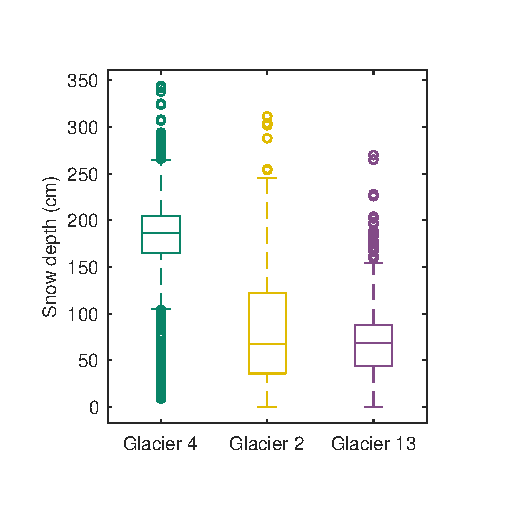
\includegraphics[width =0.5\textwidth]{DepthBoxplot.pdf}\\
	\caption{}
	\label{fig:DepthBoxplot}
\end{figure}

\begin{figure}
	\centering
	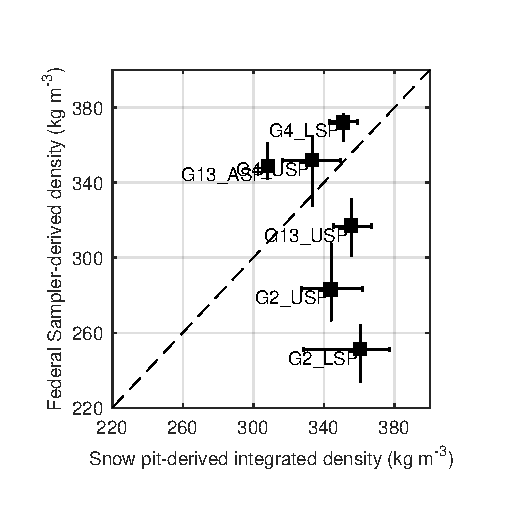
\includegraphics[width =0.5\textwidth]{SPvsFS.pdf}\\
	\caption{Comparison of integrated density estimated using wedge cutters in a snow pit and density estimated using Federal Sampler measurements for Glacier 4 (G04), Glacier 2 (G02) and Glacier 13 (G13). Snow pits were distributed in the accumulation area (ASP), upper ablation area (USP) and lower ablation area (LSP). Error bars are minimum and maximum values.}
	\label{fig:density_pitVStube}
\end{figure}

\begin{figure}
	\centering
	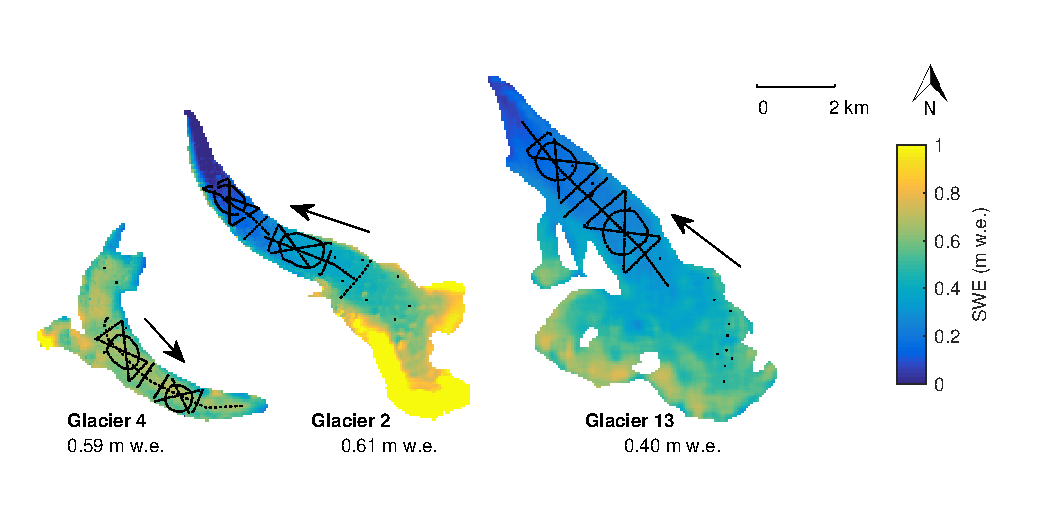
\includegraphics[width =\textwidth]{LR_map.pdf}\\
    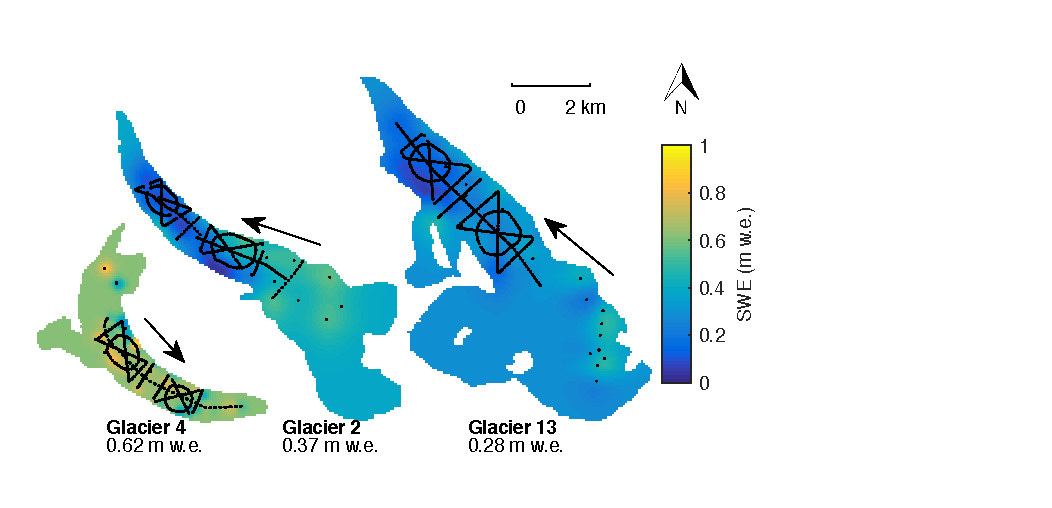
\includegraphics[width =\textwidth]{SK_map.pdf}\\
	\caption{}
	\label{fig:LR_SK_map}
\end{figure}

\begin{figure}
	\centering
	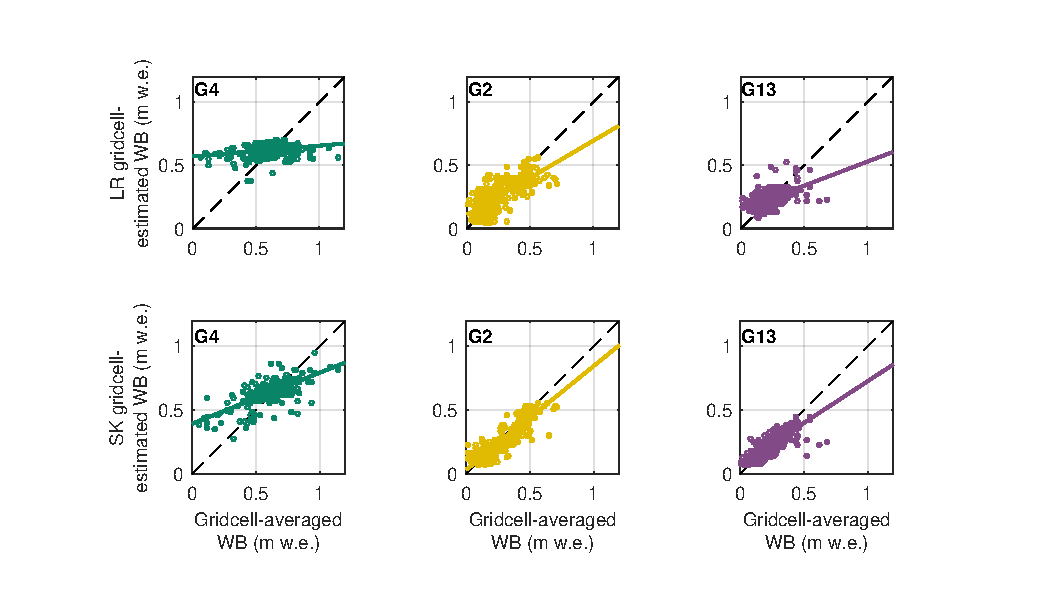
\includegraphics[width =\textwidth]{observedVSestimated_S2.pdf}\\
	\caption{}
	\label{fig:observedVSestimated_S2}
\end{figure}

\begin{figure}
	\centering
	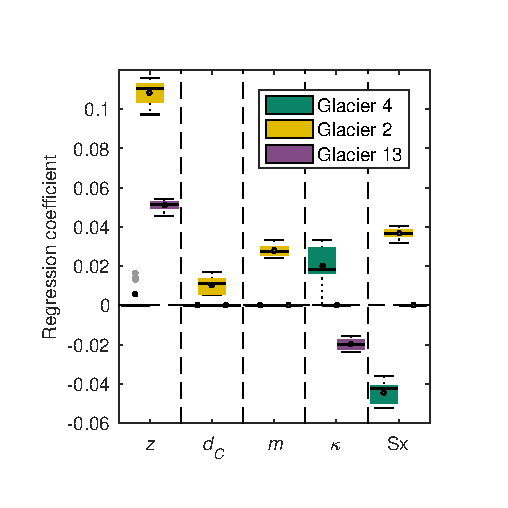
\includegraphics[width =0.5\textwidth]{BetaCoeffs.pdf}\\
	\caption{}
	\label{fig:BetaCoeffs}
\end{figure}

\begin{figure}
	\centering
	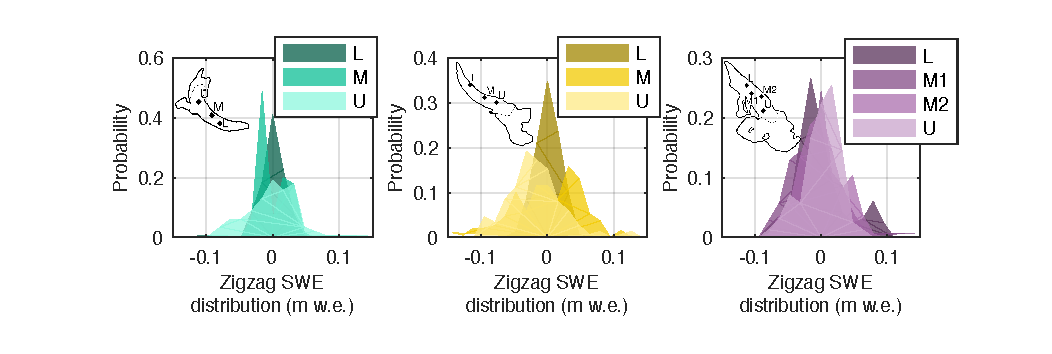
\includegraphics[width =0.5\textwidth]{ZigzagHistogram.pdf}\\
	\caption{}
	\label{fig:ZigzagHistogram}
\end{figure}


The spatial patterns and specific winter surface mass balance (WSMB) are affected by variability introduced when interpolating density, estimating grid-cell SWE values, and when interpolating observations.  


\subsection{Spatial patterns in accumulation}


\subsection{Specific winter surface mass balance (WSMB)}

The choice of interpolation method affects the mean winter balance (Figure 4.32). Kriging
interpolation produces the highest mean value of SWE on Glacier 4. The estimates of SWE
in the accumulation area are greatest when kriging is used because there is a single single
high SWE value in the accumulation area. Kriging is sensitive to outliers in areas with sparse
sampling. However, the winter balance is similar between interpolation methods and mean
of observed data for Glacier 4. This similarity arises from the low correlation coefficient for
all methods, resulting in values closer to the data mean. The observed SWE mean values
for Glaciers 2 and 13 are much lower than the estimated winter balance. Both glacier show
a significant correlation between SWE and elevation, so limiting sampling to the ablation
area skewed the observed values of SWE to be lower than the mean. Relative differences in
mean SWE between the three interpolation methods are similar for Glacier 2 and 13, with
topographic regression producing the highest mean SWE and kriging producting the lowest.
Kriging estimates lower SWE in the accumulation area of both glaciers because elevation
is not incorporated into the model.




%\begin{table}
%\caption{Example table}
%\centering
%\begin{tabular}{llr}
%\toprule
%\multicolumn{2}{c}{Name} \\
%\cmidrule(r){1-2}
%First name & Last Name & Grade \\
%\midrule
%John & Doe & $7.5$ \\
%Richard & Miles & $2$ \\
%\bottomrule
%\end{tabular}
%\end{table}

%------------------------------------------------

\section{Discussion}
[77] conducted an airborne GRP survey of two adjacent glaciers in Switzerland. The
lower part of the larger valley glacier showed a clear correlation between altitude and snow
accumulation. The upper part of the glacier and the adjacent smaller glacier had no alti-
tudinal trend and the fluctuations in depth were large. Additionally, the accumulation was
40\% lower on the smaller glacier. The altitudinal trend is a well documented pattern and
was thought to be a result of melt that occurred during warmer weather, which is more
pronounced at lower elevations. Spatial variability of precipitation and redistribution of
snow were believed to have resulted in the high spatial variability in higher parts of the
study area. Since the majority of the precipitation events originated from one direction and
the large glacier was on the lee side of a ridge, it experienced preferential deposition. Mean-
while, the smaller glacier was further along the storm track so it received less precipitation.
Overall, [77] showed that snow distribution on glaciers is not simply a function of altitude,
which corroborated research done in other alpine catchments.

 In most cases, the resolution of measurements over a large area is insufficient to
approximate the true variability [15, 32].


extrapolation of regression models will
likely result in large errors. These errors are especially relevant in the accumulation area,
which has extreme values for all parameters. Errors in the accumulation area are especially
important to acknowledge because this area has the highest values of SWE and is likely to
heavily influence final winter mass balance values. Improvements to this study could include
using an air-borne GPR to collect a dense network of SWE measurements in difficult to
access areas [e.g. 82] (see Section 1.3.2 for more details).


Lopez 2013 for small scale var

\section{Introduction}

Objective: (1) Discuss choices made when moving from measurement to accumulation and (2) show how system variability and our choices interact to create uncertainty in our estimate of accumulation

- snow distribution in alpine regions is not uniform or static, but
rather highly variable and influenced by diverse and dynamic processes operating on multiple spatial and temporal scales -> topographic effects (crevasses, surface topo, elevation aspect, precip grad across range), snow drift and preferential deposition
-  [22] note that studies of snow water equivalent (SWE) that have been conducted in
alpine environments vary considerably in the extent and spacing of their measurements.
- Snow accumulation is spatially variable on point scales (<5 m), hillslope scales (1–100 m),
basin scales (100–10,000 m) and regional scales (10–1000 km) [22].
-Point-scale variability is generally associated with surface roughness effects and the
presence of small obstacles. -> take three measures
Many parts of a glacier though
are characterized by a relatively smooth surface, with roughness lengths on the order of
centimeters [57]. In these areas, point-scale variability of snow depth is low. However, in
heavily crevassed regions, point-scale variability can be large and thus exert a dominant
control on snow distribution in the area [82].
-Hillslope-scale variability is caused by variations in the surface topography of the glacier.
The curvature and slope of the surface as well as the presence of local ridges or depressions
can affect where snow is located [15, 115]. Avalanching can also redistribute snow, especially
on the margins of a glacier [17, 89].
Watershed-scale variability results mainly from the effects of changing elevation and
aspect on atmopsheric conditions [22]. In particular, orographic lifting and shading can
result in higher elevation and north-facing areas of the glacier having more snow than other
areas [89, 115]. Gradients in temperature from elevation changes also affect the freezing
level, which determines whether precipitation falls as snow or rain [17]. For example, [77]
found a strong influence of elevation in determining accumulation on Findel Glacier in
Switzerland.
Regional variability occurs when areas within a mountain range have differing amounts of
snow. Often, this results from horizontal precipitation gradients and rain shadows forming
on the lee side of topographic divides. Areas with large, steep mountains are especially
affected by these processes.

----------------------------------------------------

derived accumulation
estimated winter surface mass balance
distributed snow water equivalent
%------------------------------------------------



%----------------------------------------------------------------------------------------
%	REFERENCE LIST
%----------------------------------------------------------------------------------------

\bibliography{/home/glaciology1/Documents/MastersDocuments/MastersLit}
\bibliographystyle{igs}

%----------------------------------------------------------------------------------------

\end{document}
